\documentclass[12pt]{article}
\usepackage{amsmath}
\usepackage{graphicx}
\usepackage{booktabs}
\usepackage{hyperref}
\usepackage{fancyhdr}
\usepackage{float}
\usepackage[margin=1in]{geometry}
\usepackage{enumitem}
\usepackage{xcolor}
\usepackage{listings}
\lstset{
  basicstyle=\ttfamily\footnotesize,
  breaklines=true,
  backgroundcolor=\color{gray!10},
  frame=single
}

\title{\textbf{Experiment 2: Loan Amount Prediction using Linear Regression}}
\author{Joice Anancia S A}
\date{July 2025}

\begin{document}
\maketitle

\section*{Aim}
To develop and evaluate a Linear Regression model that predicts the loan sanction amount using historical loan data and relevant borrower features.

\section*{Libraries Used}
\begin{itemize}
  \item Pandas: Data manipulation
  \item NumPy: Numerical operations
  \item Scikit-learn: Model building, preprocessing, and evaluation
  \item Matplotlib and Seaborn: Data visualization
\end{itemize}

\section*{Objective}
\begin{itemize}
  \item Preprocess and clean the dataset
  \item Perform exploratory data analysis (EDA)
  \item Engineer features to improve model accuracy
  \item Train and validate a Linear Regression model
  \item Evaluate model performance using MAE, MSE, RMSE, and R² metrics
  \item Visualize results and interpret model behavior
\end{itemize}

\section*{Mathematical Description}
The mathematical model for Linear Regression is:
\[
y = \beta_0 + \beta_1 x_1 + \beta_2 x_2 + \dots + \beta_n x_n + \epsilon
\]
Where:
\begin{itemize}
  \item $y$ is the dependent variable (Loan Sanction Amount)
  \item $x_1, x_2, \dots, x_n$ are the independent variables
  \item $\beta_0$ is the intercept term
  \item $\beta_1, \dots, \beta_n$ are coefficients
  \item $\epsilon$ is the error term
\end{itemize}

RSS is minimized:
\[
RSS = \sum_{i=1}^m \left( y_i - \left( \beta_0 + \sum_{j=1}^n \beta_j x_{ij} \right) \right)^2
\]

\subsection*{Evaluation Metrics}
\begin{itemize}
  \item MAE: Mean Absolute Error
  \item MSE: Mean Squared Error
  \item RMSE: Root Mean Squared Error
  \item $R^2$: Coefficient of determination
  \item Adjusted $R^2$
\end{itemize}

\section*{Python Code}
\begin{lstlisting}[language=Python]
import pandas as pd
import numpy as np
from sklearn.model_selection import train_test_split, cross_validate, KFold
from sklearn.compose import ColumnTransformer
from sklearn.preprocessing import StandardScaler, OneHotEncoder
from sklearn.pipeline import Pipeline
from sklearn.linear_model import LinearRegression
from sklearn.metrics import mean_absolute_error, mean_squared_error, r2_score
import matplotlib.pyplot as plt
import seaborn as sns

sns.set(style="whitegrid")
train_df = pd.read_csv("/content/drive/MyDrive/train.csv")
target = 'Loan Sanction Amount (USD)'

drop_cols = ['Customer ID', 'Name', 'Property ID', 'Location', 'Property Location']
train_df.drop(columns=drop_cols, inplace=True)
train_df.dropna(inplace=True)

#  Step 4: Handle missing values
train_df.dropna(inplace=True)

#  Step 5: Visualize Target Distribution
plt.figure(figsize=(8, 5))
sns.histplot(train_df[target], kde=True, color='skyblue')
plt.title('Distribution of Loan Sanction Amount')
plt.xlabel(target)
plt.ylabel('Frequency')
plt.tight_layout()
plt.show()

#  Step 6: Visualize numerical features
num_features = ['Age', 'Income (USD)', 'Credit Score', 'Dependents',
                'Current Loan Expenses (USD)', 'Property Price', 'Property Age']

for col in num_features:
    plt.figure(figsize=(8, 4))
    sns.histplot(train_df[col], kde=True, bins=30)
    plt.title(f'Distribution of {col}')
    plt.tight_layout()
    plt.show()

    plt.figure(figsize=(8, 4))
    sns.boxplot(x=train_df[col])
    plt.title(f'Boxplot of {col}')
    plt.tight_layout()
    plt.show()

#  Step 7: Correlation Heatmap
plt.figure(figsize=(10, 8))
corr_matrix = train_df[num_features + [target]].corr()
sns.heatmap(corr_matrix, annot=True, cmap='coolwarm', fmt=".2f")
plt.title('Correlation Heatmap')
plt.tight_layout()
plt.show()

#  Step 8: Scatter plots (numerical features vs target)
key_features = ['Income (USD)', 'Credit Score', 'Property Price', 'Current Loan Expenses (USD)']
for col in key_features:
    plt.figure(figsize=(8, 5))
    sns.scatterplot(data=train_df, x=col, y=target, alpha=0.6)
    plt.title(f'{col} vs {target}')
    plt.tight_layout()
    plt.show()

#  Step 9: Boxplots of categorical features vs target
cat_features = ['Gender', 'Income Stability', 'Profession', 'Type of Employment',
                'Has Active Credit Card', 'Co-Applicant', 'Property Type']

for col in cat_features:
    plt.figure(figsize=(10, 5))
    sns.boxplot(data=train_df, x=col, y=target)
    plt.title(f'{target} by {col}')
    plt.xticks(rotation=45)
    plt.tight_layout()
    plt.show()

#  Step 10: Feature Engineering
train_df['Total_Income'] = train_df['Income (USD)'] + train_df['Current Loan Expenses (USD)']
train_df['Log_Loan_Amount'] = np.log1p(train_df[target])
train_df['Log_Income'] = np.log1p(train_df['Income (USD)'])
train_df['Age_Bin'] = pd.cut(train_df['Age'], bins=[18, 30, 40, 50, 60, 100], labels=False)

#  Step 11: Define final features and target
numerical_features = ['Age', 'Income (USD)', 'Credit Score', 'Dependents',
                      'Current Loan Expenses (USD)', 'Property Price', 'Property Age', 'Total_Income']
X = train_df[numerical_features + cat_features]
y = train_df[target]

#  Step 12: Split dataset (Train=60%, Validation=20%, Test=20%)
X_train_val, X_test, y_train_val, y_test = train_test_split(X, y, test_size=0.2, random_state=42)
X_train, X_val, y_train, y_val = train_test_split(X_train_val, y_train_val, test_size=0.25, random_state=42)

#  Step 13: Preprocessing pipeline
preprocessor = ColumnTransformer([
    ('num', StandardScaler(), numerical_features),
    ('cat', OneHotEncoder(drop='first', handle_unknown='ignore'), cat_features)
])

#  Step 14: Full pipeline with Linear Regression
pipeline = Pipeline([
    ('preprocessor', preprocessor),
    ('regressor', LinearRegression())
])

#  Step 15: Train the model
pipeline.fit(X_train, y_train)

#  Step 16: Predict & Evaluate on Validation Set
y_val_pred = pipeline.predict(X_val)
mae_val = mean_absolute_error(y_val, y_val_pred)
mse_val = mean_squared_error(y_val, y_val_pred)
rmse_val = np.sqrt(mse_val)
r2_val = r2_score(y_val, y_val_pred)
adj_r2_val = 1 - (1 - r2_val) * (len(y_val) - 1) / (len(y_val) - X_val.shape[1] - 1)

print("--- Validation Metrics ---")
print(f"MAE: {mae_val:.2f}")
print(f"MSE: {mse_val:.2f}")
print(f"RMSE: {rmse_val:.2f}")
print(f"R2 Score: {r2_val:.4f}")
print(f"Adjusted R2: {adj_r2_val:.4f}")

#  Step 17: Predict & Evaluate on Test Set
y_test_pred = pipeline.predict(X_test)
mae_test = mean_absolute_error(y_test, y_test_pred)
mse_test = mean_squared_error(y_test, y_test_pred)
rmse_test = np.sqrt(mse_test)
r2_test = r2_score(y_test, y_test_pred)
adj_r2_test = 1 - (1 - r2_test) * (len(y_test) - 1) / (len(y_test) - X_test.shape[1] - 1)

print("--- Test Metrics ---")
print(f"MAE: {mae_test:.2f}")
print(f"MSE: {mse_test:.2f}")
print(f"RMSE: {rmse_test:.2f}")
print(f"R2 Score: {r2_test:.4f}")
print(f"Adjusted R2: {adj_r2_test:.4f}")

#  Step 18: Actual vs Predicted (Test Set)
plt.figure(figsize=(8, 5))
plt.scatter(y_test, y_test_pred, alpha=0.6, color='royalblue')
plt.plot([y_test.min(), y_test.max()], [y_test.min(), y_test.max()], 'r--')
plt.xlabel('Actual Loan Amount')
plt.ylabel('Predicted Loan Amount')
plt.title('Actual vs Predicted (Test Set)')
plt.tight_layout()
plt.show()

#  Step 19: Residual Plot (Test Set)
residuals_test = y_test - y_test_pred
plt.figure(figsize=(8, 5))
plt.scatter(y_test_pred, residuals_test, alpha=0.6, color='orange')
plt.axhline(0, linestyle='--', color='red')
plt.xlabel('Predicted Loan Amount')
plt.ylabel('Residuals')
plt.title('Residuals vs Predicted (Test Set)')
plt.tight_layout()
plt.show()

#  Step 20: K-Fold Cross-Validation
scoring = {
    'MAE': 'neg_mean_absolute_error',
    'MSE': 'neg_mean_squared_error',
    'R2': 'r2'
}

kf = KFold(n_splits=5, shuffle=True, random_state=42)
cv_results = cross_validate(pipeline, X, y, cv=kf, scoring=scoring)

# Convert to positive and create result table
mae_scores = -cv_results['test_MAE']
mse_scores = -cv_results['test_MSE']
rmse_scores = np.sqrt(mse_scores)
r2_scores = cv_results['test_R2']

cv_table = pd.DataFrame({
    'Fold': [f'Fold {i+1}' for i in range(5)],
    'MAE': mae_scores,
    'MSE': mse_scores,
    'RMSE': rmse_scores,
    'R2 Score': r2_scores
})

cv_table.loc['Average'] = cv_table.drop(columns='Fold').mean()
print("\n--- Cross Validation Results ---")
print(cv_table)
\end{lstlisting}

\textit{Note: Full code includes EDA, modeling, prediction, visualization, and metrics.}

\section*{Output Screenshots}
\begin{figure}[H]
      \centering
      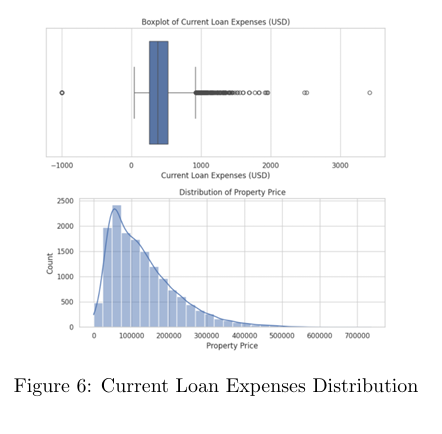
\includegraphics[width=0.5\linewidth]{image.png}
      \caption{ Figure 1: Performance Metrics}
      \label{fig:enter-label}
  \end{figure}
  
  \begin{figure}[H]
      \centering
      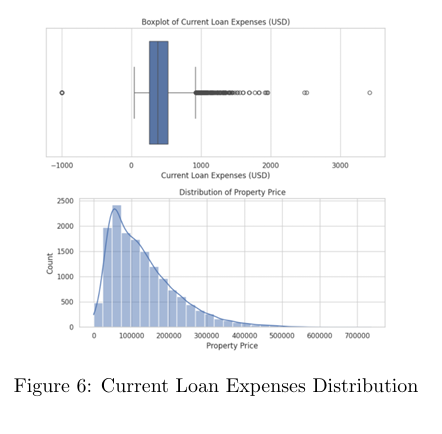
\includegraphics[width=0.5\linewidth]{image.png}
      \caption{Figure 2: Distribution of Dataset}
      \label{fig:enter-label}
  \end{figure}
    \begin{figure}[H]
        \centering
        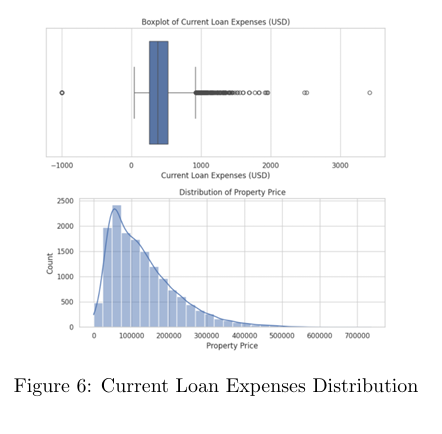
\includegraphics[width=0.5\linewidth]{image.png}
        \caption{Figure 3: Boxplot of Features}
        \label{fig:enter-label}
    \end{figure}
  \begin{figure}[H]
      \centering
      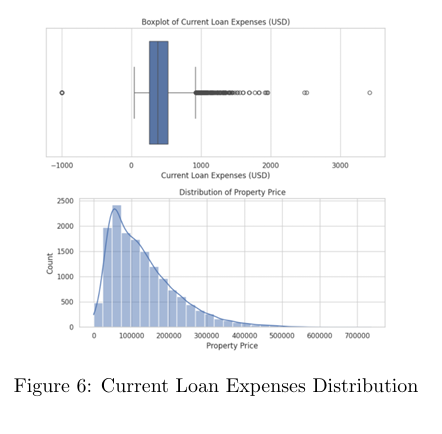
\includegraphics[width=0.5\linewidth]{image.png}
      \caption{Figure 4: Correlation Heatmap}
      \label{fig:enter-label}
  \end{figure}
  \begin{figure}[H]
      \centering
      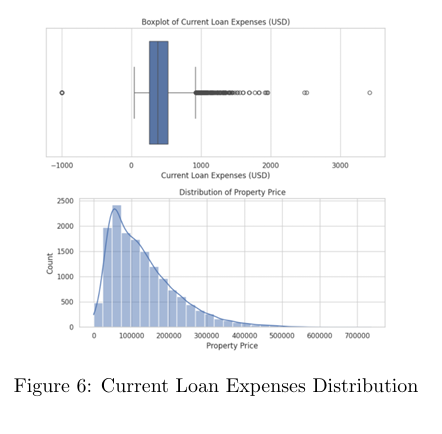
\includegraphics[width=0.5\linewidth]{image.png}
      \caption{Figure 5: Actual vs Predicted Loan Amount}
      \label{fig:enter-label}
  \end{figure}
  \begin{figure}
      \centering
      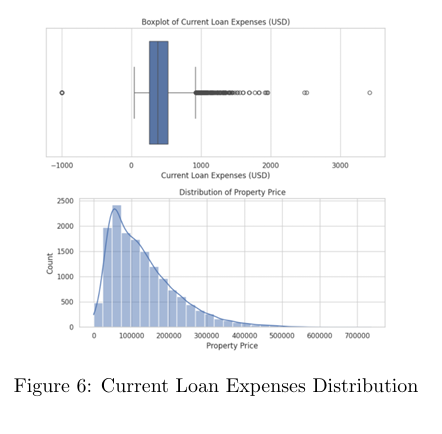
\includegraphics[width=0.5\linewidth]{image.png}
      \caption{Figure 6: Residual Plot}
      \label{fig:enter-label}
  \end{figure}
  


\section*{Inference Table}

\subsection*{Cross-Validation Results (5-Fold)}
\begin{tabular}{lcccc}
\toprule
Fold & MAE & MSE ($\times 10^8$) & RMSE & $R^2$ \\
\midrule
Fold 1 & 22090.85 & 9.96 & 31556.51 & 0.5483 \\
Fold 2 & 21386.32 & 9.40 & 30655.92 & 0.5652 \\
Fold 3 & 22128.77 & 10.8 & 32933.10 & 0.5183 \\
Fold 4 & 21838.68 & 9.65 & 31069.29 & 0.5727 \\
Fold 5 & 21917.13 & 9.55 & 30896.81 & 0.5817 \\
\midrule
Average & 21872.35 & 9.88 & 31422.33 & 0.5572 \\
\bottomrule
\end{tabular}

\vspace{1em}
\subsection*{Results Summary}
\begin{itemize}
  \item Dataset Size (after preprocessing): 15,183
  \item Train/Test Split: 60/20/20
  \item Features Used: Age, Income, Credit Score, etc.
  \item Model Used: Linear Regression
  \item Cross-Validation Folds: 5
  \item MAE (Test Set): 22145.56
  \item RMSE (Test Set): 31592.20
  \item $R^2$ (Test Set): 0.5472
  \item Adjusted $R^2$: 0.5450
\end{itemize}

\section*{Best Practices}
\begin{itemize}
  \item Handle missing values appropriately
  \item Feature engineering like log transforms and income sum
  \item Normalize numerical and encode categorical data
  \item Evaluate with multiple metrics
  \item Analyze residuals for bias
\end{itemize}

\section*{Learning Outcomes}
\begin{itemize}
  \item Understood end-to-end ML pipeline
  \item Learned feature engineering
  \item Applied cross-validation and evaluation metrics
  \item Interpreted residual and prediction plots
\end{itemize}

\end{document}
